\documentclass[conference]{IEEEtran}
\IEEEoverridecommandlockouts
% The preceding line is only needed to identify funding in the first footnote. If that is unneeded, please comment it out.
\usepackage{cite}
\usepackage{amsmath,amssymb,amsfonts}
\usepackage{algorithmic}
\usepackage{graphicx}
\usepackage{textcomp}
\usepackage{xcolor}
\usepackage{multirow}
\usepackage{makecell}
\usepackage{float}

\def\BibTeX{{\rm B\kern-.05em{\sc i\kern-.025em b}\kern-.08em
    T\kern-.1667em\lower.7ex\hbox{E}\kern-.125emX}}
\begin{document}

\title{Blood cells image segmentation and counting using deep transfer learning }

\author{
\IEEEauthorblockN{1\textsuperscript{st} Gharbi Aghiles}
\IEEEauthorblockA{\textit{University M’hamed Bougara}\\ Independence Avenue, 35000\\
Boumerdes, Algeria \\
a.gharbi@univ-boumerdes.dz}
\and
\IEEEauthorblockN{2\textsuperscript{nd} Neggazi Mohamed Lamine}
\IEEEauthorblockA{\textit{University M’hamed Bougara}\\ Independence Avenue, 35000\\
Boumerdes, Algeria \\
neggazimedlamine@gmail.com}
\and
\IEEEauthorblockN{3\textsuperscript{rd} Touazi Faycal}
\IEEEauthorblockA{\textit{University M’hamed Bougara}\\ Independence Avenue, 35000\\
Boumerdes, Algeria \\
f.touazi@univ-boumerdes.dz}
\and
\IEEEauthorblockN{4\textsuperscript{th} Yagoubi Mohamed Riad}
\IEEEauthorblockA{\textit{University M’hamed Bougara}\\ Independence Avenue, 35000\\
Boumerdes, Algeria \\
md.yagoubi@univ-boumerdes.dz}
\and
\IEEEauthorblockN{5\textsuperscript{th} Gaceb Djamel}
\IEEEauthorblockA{\textit{University M’hamed Bougara}\\ Independence Avenue, 35000\\
Boumerdes, Algeria \\
dj.gaceb@gmail.com }
}

\maketitle

\begin{abstract}
Blood cell counting is a tedious task that would benefit greatly from automation. Accurate cell counting CBC (Complete Blood Count) provides essential quantitative information and plays a key role in biological research as well as industrial and biomedical applications. Unfortunately, the commonly used manual counting method is time consuming, poorly standardized and not reproducible. The task is made even more difficult by overlapping cells and poor imaging quality. In this paper we compare between two convolutional neural networks that will segment the cells as a first phase, then count them in the second phase using 3 different algorithms (Watershed, Connected Component Labeling and Circle Hough Transform).
\end{abstract}

\begin{IEEEkeywords}
Blood cell segmentation, Blood cell counting, U-net, SegNet, deep learning 
\end{IEEEkeywords}

\section{Introduction}
Blood carries out many vital functions as it circulates through the body. It transports oxygen from the lungs to other body tissues and carries away carbon dioxide. It carries nutrients from the digestive system to the cells of the body, and carries away wastes for excretion by the kidneys. Blood helps our body fight off infectious agents and inactivates toxins, stops bleeding through its clotting ability, and regulates our body temperature. Doctors rely on many blood tests to diagnose and monitor diseases. Some tests measure the components of blood itself; others examine substances found in the blood to identify abnormal functioning of various organs. Hence, we here propose a software system which will assist pathologists to detect blood cell count and help to find out the diseases. This information can be very helpful to a physician who, for example, is trying to identify the cause of a patient's diseases.

Earlier hematologists were performing microscopic, examination and counting of blood cells manually, which was very time-consuming and tedious process. Also, the accuracy of counting mainly depends on their expertise skill and their physical conditions. Also, because of cells complex nature, it still remains a challenging task to segment cells from their background and count them automatically.

Our work is to automate the task of cell counting, we will try to find the best solution to count red, white blood cells and platelets. Therefore, we proceed in two steps:
\begin{itemize}
    \item \textbf{The segmentation:} where we need to segment the image and remove the noise to get a clear mask on which we are going preform the counting. In this phase we are comparing between two convolutional neural networks U-Net and SegNet.
    \item \textbf{The counting:} in which we will take the output mask (and edge-mask for red blood cells) from the first phase and apply counting algorithms on it. We used 3 algorithms to count the cells: Watershed, Connected Component Labeling, Circle Hough transform.\
\end{itemize}

\section{Related Work}
Bhavnani et al. \cite{bhavnani2016segmentation} have developed a method for segmenting and counting RBC (red blood cells), WBC (White blood cells) and platelets which is also called complete blood count (CBC), by using Otsu’s thresholding and morphological operations as a segmentation method, and for counting they are preforming a comparison between two methods: the watershed algorithm and Circular Hough Transform. The CHT method is the best in terms of accuracy with 92.67\% but it has some weaknesses with overlapping cells and morphological abnormalities. In the other side the watershed method which is a little bit adapted with overlapping and touching cells achieved an accuracy of 91.07\%.\

Guiliang, FENG et al.\cite{guiliang2016microscopic} have a developed an algorithm that segments and counts cell images based on image definition, a Discrete Cosine Transform (DCT) is applied, which is proposed by N. Ahmed and Rao in 1974 \cite{ahmed1974discrete}. Instead of the traditional watershed approach, the DCT method showed better results in comparison.\

However, there is a drawback to this approach, because this algorithm depends on image definition it relies on well focused images, consequently, when the images are out of focus the segmentation and counting is not reliable. But despite that drawback, it achieved a relatively high accuracy of over 90\% which is better that the watershed method.\\

K. Sudha and P. Geetha \cite{SUDHA2020639} have developed a two stage framework which will segment the leukocytes (a type of WBC) with an edge strength-based Grabcut method as a first stage, in the second stage will count the cells using the novel gradient circular hough transform (GCHT) method. the model takes and RGB image convert it to HSV color space to extract the S component where the WBCs are more clear then applies the edge strength-based location detection the results are fed to fine segmentation using Grabcut Algorithm which will output the edge segmentation mask, for the counting the mask will be fed to the proposed GCHT Algorithm. In the experiments phase they used ALL-IDB \cite{labati2011all} and Cellavision \cite{Zheng2018} datasets, after resizing the images to 256x256.\\
After the experiments the proposed method had reached an average segmentation accuracy of 99.32\% and a counting accuracy of 97.3\%.\\
The new GCHT method can segment touched cells and even overlapped cells.

Kimbahune et al. \cite{kimbahune2011blood} have developed a method for segmenting and counting red blood cells (RBC) and white blood cells (WBC).
segmentation is done using Pulse-Coupled Neural Network (PCNN) and square tracing algorithm for contour tracing after de-noising it with PCNN combined with median filter, the counting is performed by scanning the image and using edge detection methods as square tracing algorithm. this method gave good results compared to state of art methods.\\
%this kimbahune article they didn't give any info about the database or the experimental results 

Carlos X. Hern{\'{a}}ndez et al. \cite{DBLP:journals/corr/abs-1802-10548} have used a convolutional neural network (CNN) using a feature pyramid network (FPN) combined with a VGG style neural network for segmenting and counting of cells in a given microscopy image.\
The dataset they used is BBBC005 \cite{ljosa2012annotated} from Broad Institute's Bio-image Benchmark Collection, which consists of 9600 images and each image is 696x520 pixels but they were scaled down to 256x192 for the purposes of their experiment.\

Out of the total 9600 images only 600 of the images which have a corresponding mask were used for the FPN training. And 100 of those were used for fast prototyping and a standard of 80-20 train/test split for the final models.\
On the other hand, the full 9600 images were used for the VGG network.
This approach achieved a relatively good accuracy of 81.75\% but with some failure cases such as:\
%the accuracy is calculated manually from the given results in the article
% 100 - (rmspe = np.sqrt(np.mean(np.square(((y_true - y_pred) / y_true)), axis=0)))

\begin{itemize}
  \item High cell overlap
  \item Irregular cell shapes
  \item bad focal planes.
\end{itemize}

Tran, Thanh and Minh et al. \cite{tran2019blood} have developed a method for segmenting and counting RBC and WBCs by using the SegNet model initialised with weights from a pre-trained VGG-16 model, for the counting they first apply Distance transform with 4 different distance metrics, then they apply binary dilation. At the End, they apply the connected component labeling algorithm to count the number of separated cells in images mask. for the training they used 42 images from ALL-IDB1 \cite{labati2011all} after they cropped them to decrease the computation time and memory usage and reduce the number of RBC compared to WBC the result images have a resolution of 360*480*3 (RGB), they used 29 images for training and 13 for testing ,the model had a segmentation accuracy of 89\% and counting accuracy of 93.3\% on RBC and accuracy of 100\% on WBC with the testing database which has the cropped images of RBC and WBC.\

On the first database with cropped images they had only few WBC but in this second database they have more WBC , the database 2 contains 108 only WBC images with the same size of database 1 360*480*3, they augmented the training dataset from 76 to 380 and used 32 images for testing, this second model focus only on the WBC which will increase the segmentation accuracy to 98.5\%, and have a counting accuracy of 97.29\%. The counting accuracy have decreased because of the clumped cells which is the weakness of this model.

Yan Kong et al.\cite{Kong:20} have developed a two-stage framework using parallel modified U-Nets together with seed guided water-mesh algorithm for automatic segmentation and yeast cells counting which is used to observe the living conditions and survival of yeast cells under experimental conditions.\

The cell images used in this study were captured by Olympus IX83 (Olympus Life Sciences, Tokyo, Japan) inverted microscope. They manually selected 20 raw DIC (differential interference contrast) images which contained a number of yeast cells and the annotations were done manually by laboratory technicians, they then obtain 40 images, 20 masked annotation images and the other 20 is center annotation images of yeast cells.\

After splitting images into tiles of size 224x224 with a step stride of 65 and 33 pixels for the horizontal and vertical direction, respectively. They got 4360 raw image tiles and the corresponding center annotation and masked annotation images, from that set 3310 tiles were randomly selected as the training data set and rest was a validation set.

The raw test DIC images used in this study were sized approximately 1002x1998 pixels, but they were resized into 1092x2084 pixels so that each DIC image could be split into a grid of 8x16 image blocks. The image blocks were then fed into modified U-Net.

This method achieved a precision of over 99.74\% and an average recall rate of 99.35\%. however, there is a limitation using this approach, which is the detection of small objects.\\

Shahzad, Muhammad et al. \cite{shahzad2020robust} have developed a custom convolutional encoder-decoder framework along with VGG-16 as the pixel-level feature extraction model to address the problem of whole-slide cell segmentation using the semantic segmentation approach. Their proposed framework works as follows: First, all the original images along with manually generated ground truth masks of each blood cell type are passed through the pre-processing stage. In the pre-processing stage, pixel-level labeling, RGB to gray-scale conversion of masked image and pixel fusing, and unity mask generation are performed. After that, VGG16 is loaded into the system, which acts as a pre-trained pixel-level feature extraction model. Finally, the training process is initiated on the proposed model.

They used ALL-IDB1 as their baseline dataset which consists of 108 whole-slide blood cell images, 59 (2592x1944) images were from healthy individuals and 49 (1712x1368) images from acute lymphoblastic leukemia (ALL) patients.

This approach achieved a class-wise accuracy of 97.45\%, 93.34\%, and 85.11\% for RBCs, WBCs, and platelets, respectively, while global and mean accuracy remain 97.18\% and 91.96\%, respectively.\\

Overton, Toyah and Tucker, Allan \cite{10.1007/978-3-030-44584-3_31} have developed a method which segments and counts IDP (Internally Displaced people) and erythrocytes (red blood cells) using DO-U-Net (Dual Output U-Net) which outputs a segmentation mask and an edge mask then they subtract them to get rid of the overlapping and the touching problem, the model trains on extremely small datasets (10 images) and gives a high segmentation accuracy, They selected 10 images of 108 from ALL-IDB dataset for training the model, the model takes images with a resolution of 188x188 and outputs a segmentation mask and edge mask of lower resolution 100x100, the experiments results have given an accuracy of 98.31\% on a 5 randomly selected images from ALL-IDB, for the IDP they had 98.69\% for fixed resolution images and 94.66\% for scale-invariant satellite images.\\

Li, Dongming et al. \cite{li2021robust} have developed a method for segmenting blood cells by combining neural ordinary differential equations (NODEs) with U-Net networks to improve the accuracy of image segmentation. In order to study the effect of ODE-solve on the speed and accuracy of the network, the ODE-block module was added to the nine convolutional layers in the U-Net network. Firstly, blood cell images are pre-processed to enhance the contrast between the regions to be segmented; secondly, the same dataset was used for the training set and testing set to test segmentation results. Then they select the location where the ordinary differential equation block (ODE-block) module is added, select the appropriate error tolerance, and balance the calculation time and the segmentation accuracy, in order to exert the best performance.\

Finally, the error tolerance of the ODE-block is adjusted to increase the network depth, and the training NODEs-UNet network model is used for cell image segmentation. 

The experiment dataset for this model was provided by the Center for Medical Image and Signal Processing (MISP) and the Department of Pathology, Isfahan University of Medical Sciences \cite{sarrafzadeh2014selection}. MISP.rar contains 148 clear blood cell smear images with a size of 775x519 pixels. They picked up appropriate areas for convenient network training, then cropped 100 blood cell images with a size of 256x256 pixels by selecting a suitable area. To ensure the accuracy of the training model, they retained 20 images as the testing set and used the remaining 80 images to increase the dataset to 800 by data augmentation. Besides, they used a ratio of 3 : 1 as the training set and the validation set.

Using this approach to segment blood cell images in the testing set, it can achieve 95.3\% pixel accuracy and 90.61\% mean intersection over union. By comparing the U-Net and ResNet networks, the pixel accuracy of this network model is increased by 0.88\% and 0.46\%, respectively, and the mean intersection over union is increased by 2.18\% and 1.13\%, respectively.

\section{Data Description}
Dataset ALL-IDB1 is a version of ALL-IDB dataset, it is composed of 108 images (see figure \ref{img1}) collected during September, 2005. It contains about 39000 blood elements, where the lymphocytes have been labeled by expert oncologists \cite{labati2011all}. All images are in JPG format with 24 bit color depth, and a native resolution equal to 2592 × 1944, captured with a PowerShot G5 camera. The images are related to different magnifications of the microscope (ranging from 300 to 500). It can be freely downloaded from \cite{ALL_IDB_L}.

The ALL-IDB1 can be used for segmentation or classification with image processing methods or artificial intelligence models.
%segmentation is done using Pulse-Coupled Neural Network (PCNN) and square tracing algorithm for contour tracing after de-noising it with PCNN combined with median filter, the counting is performed by scanning the image and using edge detection methods as square tracing algorithm. this method gave good results compared to state of art methods.\\
\begin{figure}[h]
\centering
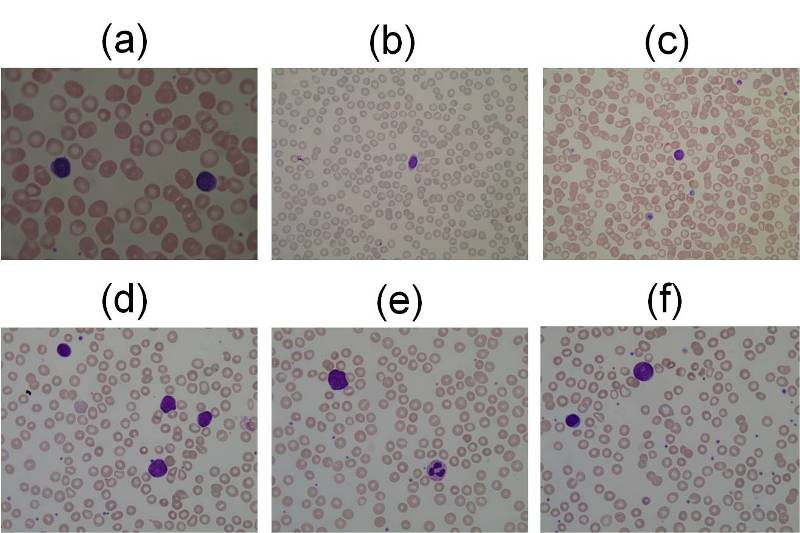
\includegraphics[width=3.5in]{images/ALLIDB1.jpg}
\caption{Examples of the images contained in ALL-IDB1: healthy cells from non-ALL patients (a,b,c), probable lymphoblasts from ALL patients (d,e,f). }
\label{img1}
\end{figure}


\section{Methodology}
U-Net and SegNet architectures are the most used in cell segmentation tasks (blood cell segmentation in particular).

In the following sections, we will briefly analyze and compare both convolutional neural network (CNN) U-Net and SegNet models with their perspective results.
And explain all the post-processing methods we used for the counting of blood cells (red, white and platelets).

\subsection{DO-U-Net}
The network is based on the fully convolutional network and its architecture was modified and extended to work with fewer training images and to yield more precise segmentations. In our case we are using DO-UNet first proposed in \cite{10.1007/978-3-030-44584-3_31} which is a modified U-Net to produce dual outputs, which is also known as a contour aware network, first demonstrated by the DCAN architecture \cite{chen2016dcan}. Based on a simple FCN, DCAN was trained to use the outer
contours of the areas of interest to guide the training of the segmentation masks. This led to improved semantic and instance segmentation of the model, which in their case, looked at non-overlapping features in biomedical imaging.
With the aim of counting closely co-located and overlapping cells, we are predominantly interested in the correct detection of individual objects as
opposed to the exact precision of the segmentation mask itself. An examination of the hidden convolutional layers of the classical U-Net showed that the penultimate layer of the network extracts information about the edges of the cells, so the idea is to output the cell mask + edge mask then do a subtraction to break the overlapping cells.

They Started with the classical U-Net then reduced the number of convolutional layers and skip connections in the model. Simultaneously, they minimised the complexity of the model by looking at smaller input regions of the images, thus minimising the memory footprint of the model. They follow the approach of Ronneberger et al. \cite{10.1007/978-3-030-44584-3_31} by using unpadded convolutions throughout the network, resulting in a model with smaller output edge and mask (100 × 100 px) corresponding to a central region of a larger (188 × 188 px) input image region. DO-U-Net uses two, independently trained, output layers of identical size. Figure \ref{fig:DO-UNET} shows the DO-U-Net architecture.

\begin{figure}
\centering
  \vspace{0.2in}
    \centerline{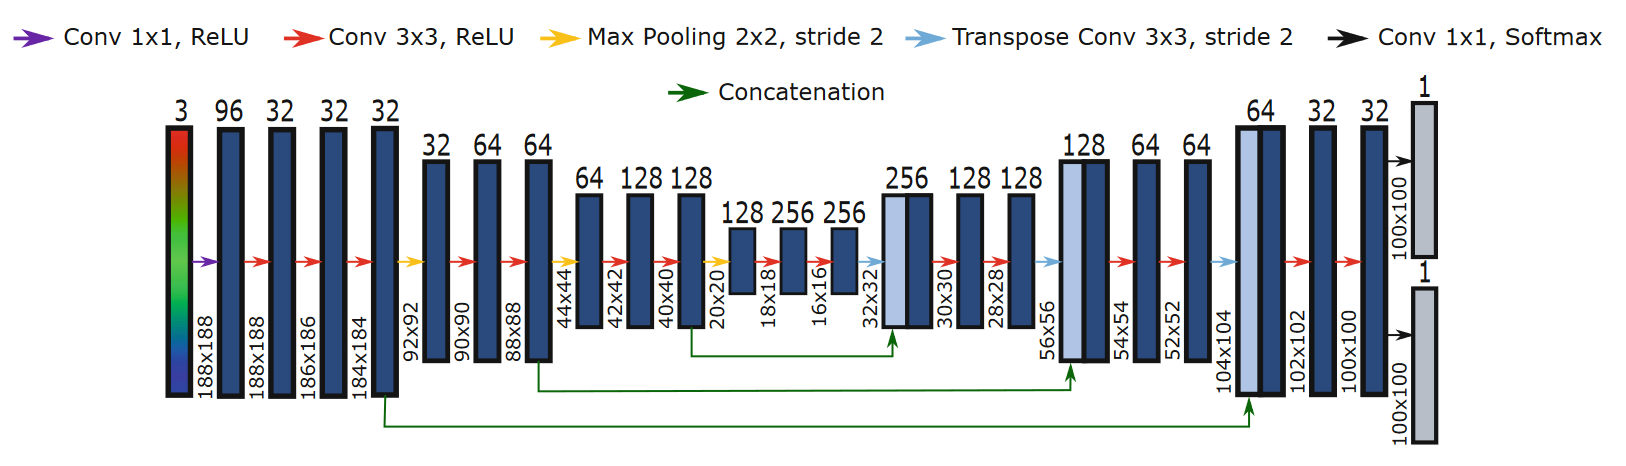
\includegraphics[width = \linewidth,height=2in]{images/DO-UNET.png}}
    \caption{DO-UNet architecture}
    \label{fig:DO-UNET}
\end{figure}

\subsection{SegNet}

The SegNet neural network, developed by Alex Kendall, Vijay Badrinarayanan, and Roberto Cipolla, all from the University of Cambridge, is a convolutional neural network used for semantic pixel wise labeling. This problem is more commonly called semantic segmentation \cite{badrinarayanan2017segnet}.

SegNet has an encoder network and a corresponding decoder network, followed by a final pixelwise classification layer. This architecture is illustrated in the figure below.
The model we used has the 13 encoder layers obtained from the VGG16 network, and 13 decoder layers to match the same number of encoder layers. The final decoder output is fed to a multi-class soft-max classifier to produce class probabilities for each pixel independently (pixelwise).

Each encoder in the encoder network performs convolution with a filter bank to produce a set of feature maps. These are then batch normalized. Then an element-wise rectified- linear non-linearity (ReLU) max(0, x) is applied. Following that, max-pooling with a 2x2 window and stride 2 (non-overlapping window) is performed and the resulting output is sub-sampled by a factor of 2. Max-pooling is used to achieve translation invariance over small spatial shifts in the input image.

The appropriate decoder in the decoder network upsamples its input feature map(s) using the memorized max-pooling indices from the corresponding encoder feature map(s). This step produces sparse feature map(s). This SegNet decoding technique is illustrated in the below figure.
These feature maps are then convolved with a trainable decoder filter bank to produce dense feature maps. A batch normalization step is then applied to each of these maps. Note that the decoder corresponding to the first encoder (closest to the input image) produces a multi-channel feature map, although its encoder input has 3 channels (RGB).
This is unlike the other decoders in the network which produces feature maps with the same number of size and channels as their encoder inputs. The high dimensional feature representation at the output of the final decoder is fed to a trainable soft-max classifier. \cite{badrinarayanan2017segnet}

The input shape we used is (128x128x3) and the output shape is (128x128), there is no loss in resolution because SegNet uses the option `same' padding on each encoder layer.
%We also tested 3 different loss functions (tversky loss, binary crossentropy and Mean Squared Error MSE), out of which the MSE outperformed the others.

\vspace{0.1in}

\begin{figure}
\centering
  \vspace{-0.1in}
    \centerline{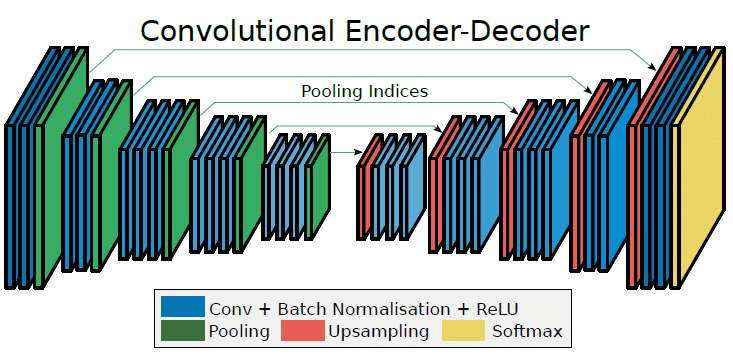
\includegraphics[width = 3in]{images/segnet.png}}
    \caption{SegNet architecture}
\end{figure}

\subsection{Dataset}
\hspace{\parindent}
For both models, we decided to work with the updated ALL-IDB1 dataset which has 13 edge-masks and 108 masks of Red Blood Cells (RBCs), 108 masks of White Blood Cells (WBCs) and Platelets. For the count information we have 13 RBC images which have the count information, but for WBCs and Platelets we had to use manual count and algorithms to find the count information because they didn't provide the count information. For the WBC we used manual count, for the Platelets we used the connected component labeling on the ground truth mask.\

10 images with their perspective masks and edge masks were chosen for red blood cell training and 3 as a test dataset, for white blood cells we used 73 images with their masks as a train dataset, and 33 as a test dataset.
For platelets, we used 71 for training and 31 as a test dataset.
Only red blood cells have edge masks, because we need to get rid of overlapped cells, white blood cells and platelets don't need the edge masks, we can retrieve all the necessary features using masks only, because both white blood cells and platelets rarely overlap.
The images will be sliced to the input size of the according model to match the input shape of the models, we also add a padding when we slice to recover the edges loss in convolution.
The resulting train dataset will be 3916 image, mask, and edge tiles (a total of 11748 tiles) see table \ref{table:total_tiles}.
For the test dataset 1072 image, mask, and edge tiles (a total of 3216 tiles) for red blood cells.
As for white blood cells, 28126 image and mask tiles were used for training (a total of 56252 tiles), and 15892 image and mask tiles were used as a test dataset for white blood cells (a total of 31784 tiles).
Finally, for platelets we used 27650 image and mask tiles were used for training (a total of 55300), and 14410 image and mask tiles as a test dataset for platelets (a total of 28820).\\
Here is a table which contains the resulting sliced images for red blood cells, white blood cells and platelets:

\begin{table}[H]
\centering
\resizebox{\columnwidth}{!}{%
\begin{tabular}{|cc|c|c|c|c|c|c|}
\hline
\multicolumn{2}{|c|}{{\color[HTML]{000000} \textbf{Dataset}}}                                                                     & {\color[HTML]{000000} \textbf{\begin{tabular}[c]{@{}c@{}}Train\\ images\end{tabular}}} & {\color[HTML]{000000} \textbf{\begin{tabular}[c]{@{}c@{}}Test\\ images\end{tabular}}} & {\color[HTML]{000000} \textbf{\begin{tabular}[c]{@{}c@{}}Train\\ Tiles\end{tabular}}} & {\color[HTML]{000000} \textbf{\begin{tabular}[c]{@{}c@{}}Test\\ Tiles\end{tabular}}} & {\color[HTML]{000000} \textbf{\begin{tabular}[c]{@{}c@{}}Total\\ images\end{tabular}}} & {\color[HTML]{000000} \textbf{\begin{tabular}[c]{@{}c@{}}Total\\ tiles\end{tabular}}} \\ \hline
\multicolumn{1}{|c|}{{\color[HTML]{000000} }}                                             & {\color[HTML]{000000} \textbf{Image}} & {\color[HTML]{000000} 10}                                                              & {\color[HTML]{000000} 3}                                                              & {\color[HTML]{000000} 3916}                                                           & {\color[HTML]{000000} 1072}                                                          & {\color[HTML]{000000} 13}                                                              & {\color[HTML]{000000} \textbf{4988}}                                                  \\ \cline{2-8} 
\multicolumn{1}{|c|}{{\color[HTML]{000000} }}                                             & {\color[HTML]{000000} \textbf{Mask}}  & {\color[HTML]{000000} 10}                                                              & {\color[HTML]{000000} 3}                                                              & {\color[HTML]{000000} 3916}                                                           & {\color[HTML]{000000} 1072}                                                          & {\color[HTML]{000000} 13}                                                              & {\color[HTML]{000000} \textbf{4988}}                                                  \\ \cline{2-8} 
\multicolumn{1}{|c|}{\multirow{-3}{*}{{\color[HTML]{000000} \textbf{Red Blood Cells}}}}   & {\color[HTML]{000000} \textbf{Edge}}  & {\color[HTML]{000000} 10}                                                              & {\color[HTML]{000000} 3}                                                              & {\color[HTML]{000000} 3916}                                                           & {\color[HTML]{000000} 1072}                                                          & {\color[HTML]{000000} 13}                                                              & {\color[HTML]{000000} \textbf{4988}}                                                  \\ \hline
\multicolumn{1}{|c|}{{\color[HTML]{000000} }}                                             & {\color[HTML]{000000} \textbf{Image}} & {\color[HTML]{000000} 73}                                                              & {\color[HTML]{000000} 33}                                                             & {\color[HTML]{000000} 28126}                                                          & {\color[HTML]{000000} 15892}                                                         & {\color[HTML]{000000} 106}                                                             & {\color[HTML]{000000} \textbf{44018}}                                                 \\ \cline{2-8} 
\multicolumn{1}{|c|}{\multirow{-2}{*}{{\color[HTML]{000000} \textbf{White Blood Cells}}}} & {\color[HTML]{000000} \textbf{Mask}}  & {\color[HTML]{000000} 73}                                                              & {\color[HTML]{000000} 33}                                                             & {\color[HTML]{000000} 28126}                                                          & {\color[HTML]{000000} 15892}                                                         & {\color[HTML]{000000} 106}                                                             & {\color[HTML]{000000} \textbf{44018}}                                                 \\ \hline
\multicolumn{1}{|c|}{{\color[HTML]{000000} }}                                             & {\color[HTML]{000000} \textbf{Image}} & {\color[HTML]{000000} 71}                                                              & {\color[HTML]{000000} 31}                                                             & {\color[HTML]{000000} 27650}                                                          & {\color[HTML]{000000} 14410}                                                         & {\color[HTML]{000000} 102}                                                             & {\color[HTML]{000000} \textbf{42060}}                                                 \\ \cline{2-8} 
\multicolumn{1}{|c|}{\multirow{-2}{*}{{\color[HTML]{000000} \textbf{Platelets}}}}         & {\color[HTML]{000000} \textbf{Mask}}  & {\color[HTML]{000000} 71}                                                              & {\color[HTML]{000000} 31}                                                             & {\color[HTML]{000000} 27650}                                                          & {\color[HTML]{000000} 14410}                                                         & {\color[HTML]{000000} 102}                                                             & {\color[HTML]{000000} \textbf{42060}}                                                 \\ \hline
\end{tabular}%
}
\caption{Dataset used for both models}
\label{Dataset used for both models}
\end{table}


\subsection{Dataset augmentation}
\hspace{\parindent}
We used the same dataset augmention on all cells (red, white blood cells, and platelets) in both models UNet and SegNet.
The augmentation we used was custom which involves the following steps:
\begin{enumerate}
    \item Pick a random image from the train dataset.
    \item Get the x and y coordinates randomly from the chosen image.
    \item Rescale the image randomly to a smaller size then scale it back to the original size to reduce quality.
    \item Take a slice of the image and mask accordingly and also edge if available.
    \item Skip the image if it dosn't contain out object of interest
    \item Resize the image and mask to the model input.
    \item Randomly rotate and flip the image chip.
    \item Randomly augment the colors (luminosity and saturation).
\end{enumerate}

\begin{figure}[H]
\centering
  \vspace{-0.1in}
    \centerline{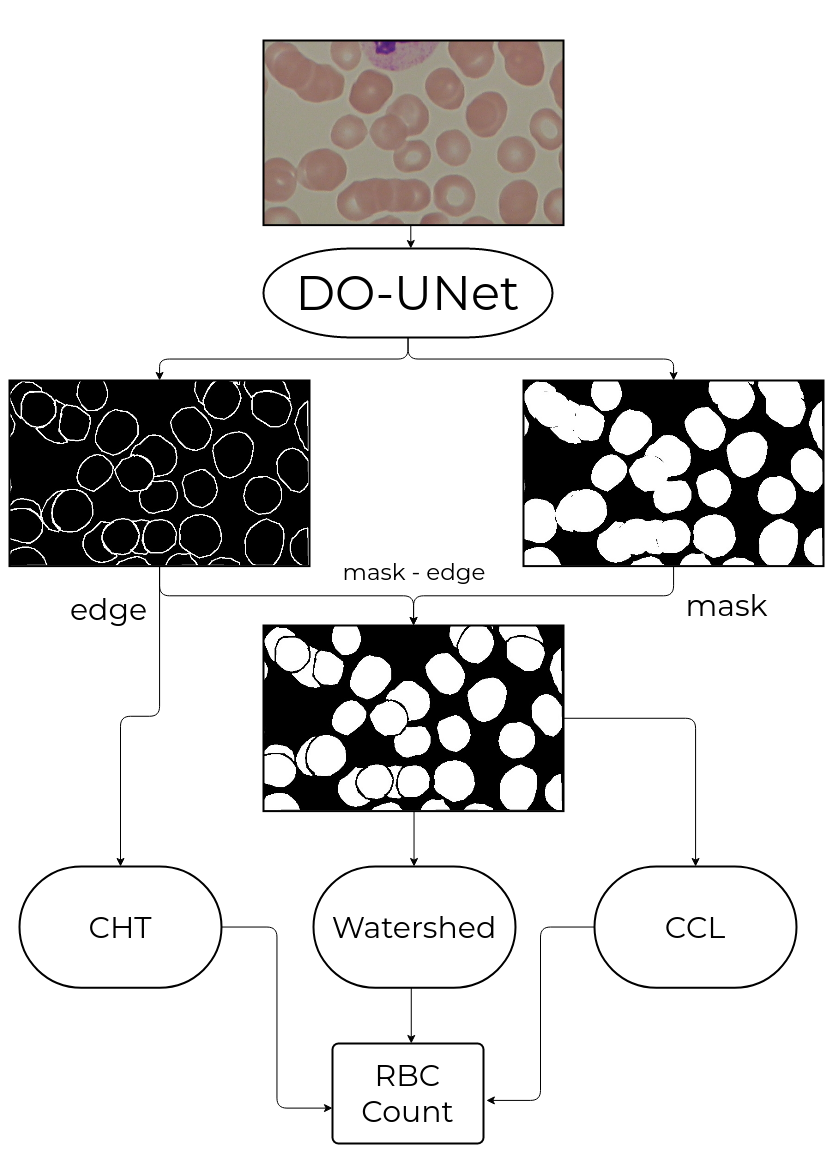
\includegraphics[width = 3in]{images/Diag_RBC_DOUNET_SegNet.png}}
    \caption{Schema of the segmentation and counting steps of the RBC's}
    \label{fig:scheme_RBC}
\end{figure}

\begin{figure}[H]
\centering
    \centerline{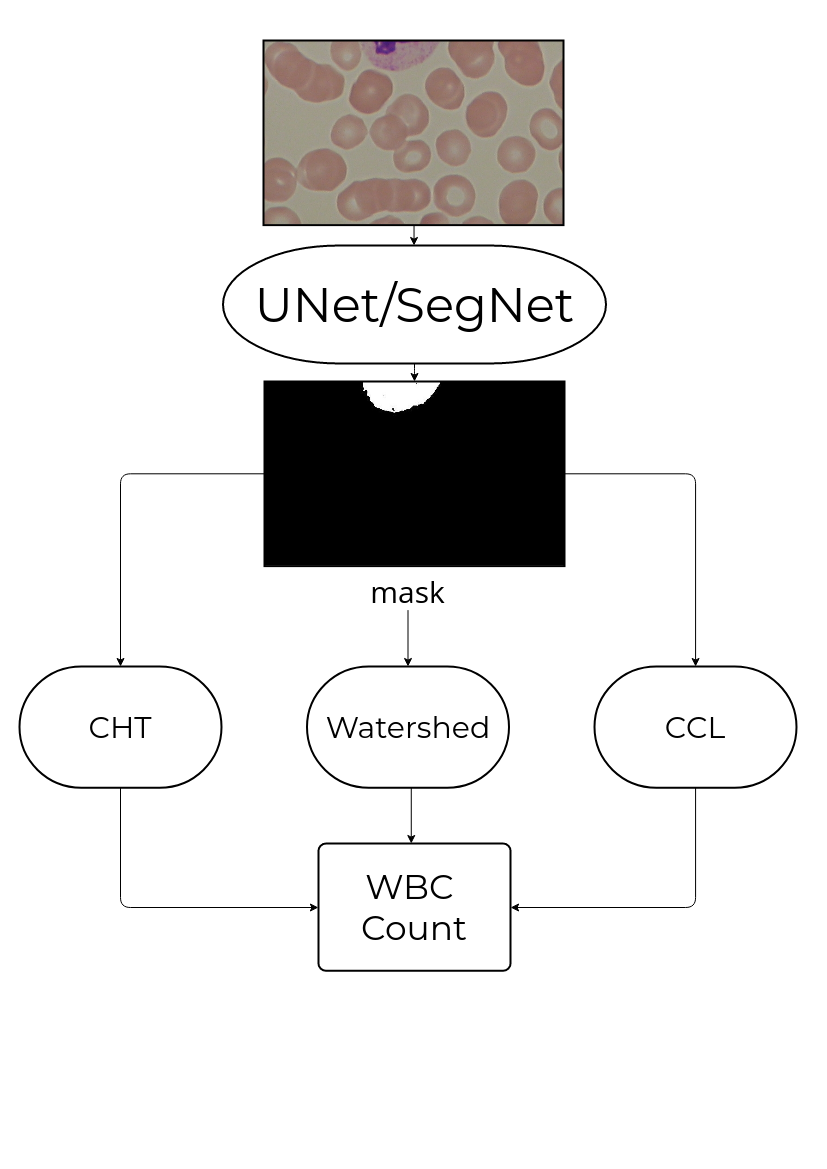
\includegraphics[width = 3in]{images/Diag_WBC_PLT_UNET_SegNet.png}}
    \caption{Schema of the segmentation and counting steps of the WBC's and Platelets}
    \label{fig:scheme_WBC_PLT}
\end{figure}

\section{Results}
\subsection{DO-U-Net Results}
\subsubsection{Red Blood Cells}
\hspace{\parindent}
They are the most difficult to detect because of their nature of overlapping, where in some samples we can't see the overlapping by the naked eye, in this experiment we are testing the DO-U-Net from \cite{10.1007/978-3-030-44584-3_31}.
For the DO-U-Net we updated the data augmentation phase, and applied Transfer Learning to get a better edge-mask. we can see in the dataset that we only have 13 images out of 108 from ALL-IDB1 that contains edge-masks and 108 masks. Consequently, there is a lack of the edge-mask labels.
We ended up with the method below as the best fit to our problem:

\begin{enumerate}
    \item Train the DO-U-Net outputs on the large dataset (108 masks) which will output two identical masks.
    \item Continue Training the DO-U-Net with the small dataset (13 masks, 13 edges), and Freeze the Mask Output.
\end{enumerate}

The table \ref{table:do-unet-transfer} compares between the normal trained model A on the small dataset which contains 13 masks and edge-masks and the model B which is trained on two phases, first using the large dataset (108 masks without edge-masks) for 60 epochs, and in the second phase we continued training using the small dataset (13 masks + edges) for 400 epochs.
We can see that this method pushed the edge accuracy higher, which is really important to get rid of the overlapping.

% 
% \usepackage{multirow}


\begin{table}[H]
\centering
\resizebox{\textwidth}{!}{\begin{tabular}{|c|l|c|c|c|c|c|c|c|} 
\hline
\textbf{RBC\_Model}  & \textbf{Dataset}                                                                                                                                & \textbf{Epochs}                                                                      & \textbf{Output}      & \textbf{Loss}        & \textbf{Mean IOU}    & \textbf{Dice}        & \textbf{Tversky}     & \textbf{Accuracy}     \\ 
\hline
\multirow{2}{*}{A}   & \multirow{2}{*}{\begin{tabular}[c]{@{}l@{}}small Dataset\\(mask + edge) * (10 + 3)\end{tabular}}                                                & \multirow{2}{*}{800}                                                                 & Mask                 & 0.3615               & 0.6365               & 0.8304               & 0.8232               & 0.8754                \\ 
\cline{4-9}
                     &                                                                                                                                                 &                                                                                      & Edge                 & 0.1816               & 0.0663               & 0.3582               & 0.3475               & 0.9343                \\ 
\hline
\multirow{2}{*}{B}   & \multirow{2}{*}{\begin{tabular}[c]{@{}l@{}}\makecell{Phase 1: large dataset mask*108\\Phase 2: small Dataset (mask + edge)*13}\end{tabular}} & \multirow{2}{*}{\begin{tabular}[c]{@{}l@{}}Phase 1: 120 \\Phase 2: 400\end{tabular}} & Mask                 & 0.0713               & 0.7751               & 0.9528               & 0.9567               & 0.9716                \\ 
\cline{4-9}
                     &                                                                                                                                                 &                                                                                      & Edge                 & 0.1465               & 0.0759               & 0.4127               & 0.4015               & 0.9385                \\ 
\hline
\multicolumn{1}{l}{} & \multicolumn{1}{l}{}                                                                                                                            & \multicolumn{1}{l}{}                                                                 & \multicolumn{1}{l}{} & \multicolumn{1}{l}{} & \multicolumn{1}{l}{} & \multicolumn{1}{l}{} & \multicolumn{1}{l}{} & \multicolumn{1}{l}{} 
\end{tabular}}
\caption{Normal trained modes compared to transfer learning model}
\label{table:do-unet-transfer}
\end{table}

After training the DO-U-Net model we did a benchmark on the 13 images to calculate the counting accuracy of the three methods, we ended up with the results below where we can see that the circle hough transform method is the best for RBC counting with 95.36 accuracy, because all the RBCs have a similar shape and size.

\subsubsection{White Blood Cells}
\hspace{\parindent}
The White Blood Cells are also difficult to detect because of the non stable shape and in some cases they overlap, in this experiment we are comparing single output U-Net from \cite{10.1007/978-3-030-44584-3_31} and the single output SegNet model.
In the U-Net we removed the edge output because we don't have the edge annotation. then trained the model for 15 epochs with the binaryCrossEntropy Loss function on (74 + 34) images. 
We ended up with a very high accuracy and IOU score as we can see in table \ref{table:unet-wbc-training}.

After training the model we did a benchmark on the 13 images then on the complete database (108 images) to calculate the counting accuracy of the three methods.\\ 
The real count of the 108 images is calculated manually because the original database doesn't have the count information. We ended up with the table \ref{table:UNet-WBC} below where we can see that the watershed method is the best for WBC counting with 97.94 accuracy on the 13 images and 95.64 on the complete database, because the white blood cells always slightly overlap each other where it's easy to the watershed to segment them.

\subsubsection{platelets}
\hspace{\parindent}
The platelets are easy to count because of the rare overlapping but they are a bit difficult to segment because of their small size.\\
In this experiment we are testing single output U-Net from \cite{10.1007/978-3-030-44584-3_31}. In the U-Net we removed the edge output because we don’t have the edge annotation.
then trained the model for 50 epochs with the BinaryCrossEntropy Loss function on (74 + 34) images.
We ended up with a very high accuracy and IOU score as we can see in table \ref{table:PLT_DOUNET_TRAIN}.

After training the model we did a benchmark on the 13 images to calculate the counting accuracy of the three methods.
We are comparing to the real count which is calculated by feeding the ground truth platelets masks to the CCL algorithm. because the original database doesn't have the count information.\\
We ended up with the table \ref{table:PLT_UNET_RESULT} below where we can see that the CCL method is the best for WBC counting with 98.58 accuracy, because of the rare overlapping on each other where it’s easy to the CCL to segment them.

\subsection{SegNet Results}
\hspace{\parindent}
SegNet segmentation results were pretty accurate for white blood cells and platelets, as for red blood cells, the segmentation was done using dual output (mask and edge-mask) to get rid of overlapped cells.\\
Here are the results of the Mean Squared Error (MSE) loss function on each type of cell:


\subsubsection{Red Blood Cells}
\hspace{\parindent}
For the dual-output SegNet model, the resulting segmented images were very good, sometimes better than the do-U-Net, though it is not as optimized when training and also predicting images, but it gets the job done with 95.86\% mask and 93.99\% edge accuracies. The segmented output images also had some noise which affected Connected Component Labeling (CCL) when counting.
As for Circle Hough Transform (CHT), the noise did not affect the result.
Red Blood Cells detection and counting is by far the hardest, because it is the only cell that overlaps and that makes it hard for counting.
The segmented output of do-SegNet is thresholded using a binary threshold, and then sent to 3 algorithms:

\begin{itemize}
  \item \textbf{Circle Hough Transform}: CHT was our best result for red blood cells counting, which achieved an accuracy of 94.03\% on the same dataset used for training the model (13 images with their respective masks and edge-masks).
  \item \textbf{Connected Component Labeling}: CCL was applied directly on the thresholded output edge, this method was far from accurate because the do-SegNet output had some noise (even when removing most of it), and also the overlapped nature of red blood cells which makes it very hard for this algorithm to count correctly. CCL achieved an accuracy of 76.49\% counting red blood cells.
  \item \textbf{Euclidean Distance Transform}: EDT is used to get rid of the overlapped cells, also peak local max was applied on the EDT output for finding local maxima(s), the result of this approach is 84.64\% accuracy.
\end{itemize}


\subsubsection{White Blood Cells}
\hspace{\parindent}
The results of white blood cells segmentation and counting using the SegNet model was very accurate achieving 99.72\% when segmenting.
White blood cells are the easiest out of the three, and the most accurate results.
However, white blood cells are different from the other cells because they come in different shapes and sizes, which made it hard to adapt each counting algorithm to every cell.\
The same counting methods are applied CHT, CCL and EDT. And each method had some drawbacks.\\
Here are the results:

\begin{itemize}
  \item \textbf{Circle Hough Transform}: Due to the different shapes of white blood cells, CHT achieved the lowest result which is 79.9\% counting accuracy, because some of the cells don't even look like circles and also their different size which made it harder to count.
  \item \textbf{Connected Component Labeling}: CCL is similar to CHT when it comes to white blood cells. And, because of the noisy outputs of SegNet the binary threshold can only do so much (it thresholds some of the noise generated when predicting).\\
    CCl achieved an average counting accuracy of 82.89\%.
  \item \textbf{Euclidean Distance Transform}: EDT is the contender of white blood cells counting, because the distance transform gets rid of the noise completely and peak local max was very helpful in eliminating that noise and getting an accurate count.\\
    This method achieved a counting accuracy of 96.43\%.
\end{itemize}

\subsubsection{Platelets}
\hspace{\parindent}
The platelets segmentation result we achieved is not the best compared to the do-U-Net model. SegNet extracts the platelets but with some noise which made it very hard to count accurately.
It achieved a segmentation accuracy of 99.89\% and the highest counting accuracy is 71.56\% which is not very good.\\
Here are all the counting accuracies for each approach:

\section{Conclusion}

In the present work, we have mainly presented two different models of segmentation based on CNNs and three counting algorithms to perform a complete blood count.
We focused more on the segmentation task where  we tested two models U-Net and SegNet to get better masks. 

We can see that the U-Net gave better result with less noisy mask, but the two models has some weaknesses with the images color space, because both models takes rgb images therefore they depend a lot on the color features, for example if we slightly change the colors of the input image we get a big diffrence in the output mask.
In the counting task, we had a small time window where we couldn't tune the 3 three algorithm parameters to get the best results. but we got acceptable results in each blood cell type, especially with platelets.\\

As a future work, we can combine between the two models to benefit the strength points of both models, we can also find more combinations between edge and mask.

\bibliographystyle{IEEEtran}
\bibliography{main}

\end{document}
